\section{Hàm số $y=ax^2$ ($a\ne0$)}

\begin{lesson}
    \subsection{Kiến thức trọng tâm}

    \textbf{Mở đầu.} Một cây cầu treo có trụ tháp đôi cao $75$ m so với mặt của cây cầu và cách nhau $400$ m. Các dây cáp có dạng đồ thị của hàm số $y=ax^2$ ($a\ne0$) như Hình 6.1 và được treo trên các đỉnh tháp. Tìm chiều cao $CH$ của dây cáp biết điểm $H$ cách tâm $O$ của cây cầu $100$ m (giả sử mặt của cây cầu là bằng phẳng).

    \begin{center}
    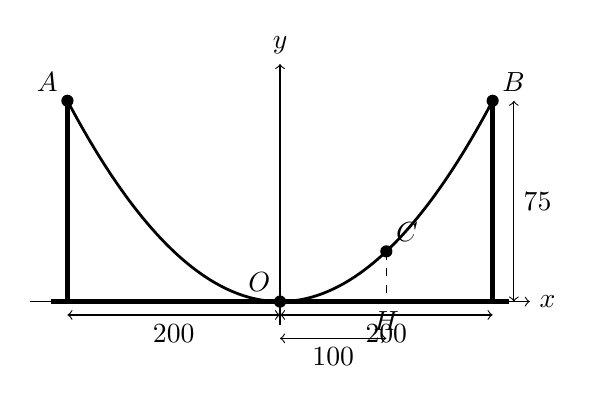
\begin{tikzpicture}[x=1.35cm,y=0.85cm]
        \coordinate (O) at (0,0);
        \coordinate (A) at (-2,3);
        \coordinate (B) at (2,3);
        \coordinate (H) at (1,0);
        \coordinate (C) at (1,0.75);

        \draw[->] (-2.35,0) -- (2.35,0) node[right] {$x$};
        \draw[->] (0,-0.35) -- (0,3.55) node[above] {$y$};
        \draw[line width=2pt] (-2.15,0) -- (2.15,0);
        \draw[line width=2pt] (-2,0) -- (A);
        \draw[line width=2pt] (2,0) -- (B);
        \draw[domain=-2:2,samples=81,smooth,variable=\x,line width=1pt]
            plot ({\x},{0.75*(\x)^2});
        \draw[dashed] (C) -- (H);

        \fill (A) circle[radius=2.2pt] node[above left] {$A$};
        \fill (B) circle[radius=2.2pt] node[above right] {$B$};
        \fill (O) circle[radius=2.2pt] node[above left] {$O$};
        \fill (C) circle[radius=2.2pt] node[above right] {$C$};
        \node[below] at (H) {$H$};

        \draw[<->] (-2,-0.2) -- (0,-0.2) node[midway,below] {$200$};
        \draw[<->] (0,-0.2) -- (2,-0.2) node[midway,below] {$200$};
        \draw[<->] (0,-0.55) -- (1,-0.55) node[midway,below] {$100$};
        \draw[<->] (2.2,0) -- (2.2,3) node[midway,right] {$75$};
    \end{tikzpicture}

    \textit{Hình 6.1}
    \end{center}

    \textbf{1. HÀM SỐ $y=ax^2$ ($a\ne0$)}

    \textbf{Nhận biết hàm số $y=ax^2$ ($a\ne0$)}

    \textbf{HĐ1.} Khi thả một vật rơi tự do và bỏ qua sức cản của không khí, quãng đường chuyển động $s$ (mét) của vật được cho bằng công thức $s=4{,}9t^2$, trong đó $t$ (giây) là thời gian chuyển động của vật.
    \begin{enumerate}[label=\alph*)]
        \item Hoàn thành bảng sau vào vở:

        \begin{center}
        \begin{tblr}{
            colspec={Q[c] *{3}{Q[c]}},
            rows={0.9cm}
        }
            $t$ (giây) & $0$ & $1$ & $2$ \\
            $s$ (m) & & & \\
        \end{tblr}
        \end{center}

        \item Giả sử một vật rơi tự do từ độ cao $19{,}6$ m so với mặt đất. Hỏi sau bao lâu vật chạm đất?
    \end{enumerate}

    \answerline

    \textbf{HĐ2.}
    \begin{enumerate}[label=\alph*)]
        \item Viết công thức tính diện tích $S$ của hình tròn bán kính $r$.
        \item Hoàn thành bảng sau vào vở (lấy $\pi=3{,}14$ và làm tròn kết quả đến chữ số thập phân thứ hai):

        \begin{center}
        \begin{tblr}{
            colspec={Q[c] *{4}{Q[c]}},
            rows={0.9cm}
        }
            $r$ (cm) & $1$ & $2$ & $3$ & $4$ \\
            $S$ (cm$^2$) & & & & \\
        \end{tblr}
        \end{center}
    \end{enumerate}

    Những công thức tính $s$ theo $t$ (trong HĐ1), tính $S$ theo $r$ (trong HĐ2) biểu thị những hàm số có cùng một dạng, gọi là hàm số $y=ax^2$ ($a\ne0$).

    \begin{keyconcept}
        \textbf{Nhận xét.} Hàm số $y=ax^2$ ($a\ne0$) xác định với mọi giá trị $x$ thuộc $\mathbb{R}$.
    \end{keyconcept}

    \textbf{Ví dụ 1.} Cho hàm số $y=\dfrac{3}{2}x^2$. Hoàn thành bảng giá trị sau vào vở:

    \begin{center}
    \begin{tblr}{
        colspec={Q[c] *{7}{Q[c]}},
        rows={0.9cm}
    }
        $x$ & $-3$ & $-2$ & $-1$ & $0$ & $1$ & $2$ & $3$ \\
        $y=\dfrac{3}{2}x^2$ & & & & & & & \\
    \end{tblr}
    \end{center}

    \textbf{Giải}

    Bảng giá trị:

    \begin{center}
    \begin{tblr}{
        colspec={Q[c] *{7}{Q[c]}},
        rows={0.9cm}
    }
        $x$ & $-3$ & $-2$ & $-1$ & $0$ & $1$ & $2$ & $3$ \\
        $y=\dfrac{3}{2}x^2$ & $\dfrac{27}{2}$ & $6$ & $\dfrac{3}{2}$ & $0$ & $\dfrac{3}{2}$ & $6$ & $\dfrac{27}{2}$ \\
    \end{tblr}
    \end{center}

    \textbf{Luyện tập 1.} Cho hàm số $y=-\dfrac{3}{2}x^2$. Hoàn thành bảng giá trị sau vào vở:

    \begin{center}
    \begin{tblr}{
        colspec={Q[c] *{7}{Q[c]}},
        rows={0.9cm}
    }
        $x$ & $-3$ & $-2$ & $-1$ & $0$ & $1$ & $2$ & $3$ \\
        $y=-\dfrac{3}{2}x^2$ & & & & & & & \\
    \end{tblr}
    \end{center}

    \textbf{Vận dụng 1.} Cho hình chóp tứ giác đều có đáy là hình vuông cạnh $a$ (cm) và chiều cao $15$ cm.
    \begin{enumerate}[label=\alph*)]
        \item Viết công thức tính thể tích $V$ của hình chóp theo $a$ và tính giá trị của $V$ khi $a=5$ cm.
        \item Nếu độ dài cạnh đáy tăng lên hai lần thì thể tích của hình chóp thay đổi thế nào?
    \end{enumerate}

    \answerline
    \answerline

    \textbf{2. ĐỒ THỊ CỦA HÀM SỐ $y=ax^2$ ($a\ne0$)}

    \textbf{Cách vẽ đồ thị hàm số $y=ax^2$ ($a\ne0$)}

    \textbf{HĐ3.} Cho hàm số $y=2x^2$.
    \begin{enumerate}[label=\alph*)]
        \item Hoàn thành bảng giá trị sau vào vở:

        \begin{center}
        \begin{tblr}{
            colspec={Q[c] *{7}{Q[c]}},
            rows={0.9cm}
        }
            $x$ & $-3$ & $-2$ & $-1$ & $0$ & $1$ & $2$ & $3$ \\
            $y=2x^2$ & & & & & & & \\
        \end{tblr}
        \end{center}

        \item Trong một mặt phẳng tọa độ $Oxy$, biểu diễn các điểm $(x;y)$ trong bảng giá trị ở câu a. Bằng cách làm tương tự, lấy nhiều điểm $(x;2x^2)$ với $x\in\mathbb{R}$ và nối lại, ta được đồ thị của hàm số $y=2x^2$.
    \end{enumerate}

    \begin{keyconcept}
        \textbf{Cách vẽ đồ thị hàm số $y=ax^2$ ($a\ne0$)}
        \begin{itemize}
            \item Lập bảng ghi một số cặp giá trị tương ứng của $x$ và $y$.
            \item Trong mặt phẳng tọa độ $Oxy$, biểu diễn các cặp điểm $(x;y)$ trong bảng giá trị trên và nối chúng lại để được một đường cong là đồ thị của hàm số $y=ax^2$ ($a\ne0$).
        \end{itemize}
    \end{keyconcept}

    \textbf{Ví dụ 2.} Vẽ đồ thị của hàm số $y=-\dfrac{1}{4}x^2$.

    \textbf{Giải}

    Lập bảng một số giá trị tương ứng của $x$ và $y$:

    \begin{center}
    \begin{tblr}{
        colspec={Q[c] *{7}{Q[c]}},
        rows={0.9cm}
    }
        $x$ & $-4$ & $-2$ & $-1$ & $0$ & $1$ & $2$ & $4$ \\
        $y=-\dfrac{1}{4}x^2$ & $-4$ & $-1$ & $-\dfrac{1}{4}$ & $0$ & $-\dfrac{1}{4}$ & $-1$ & $-4$ \\
    \end{tblr}
    \end{center}

    Biểu diễn các điểm $(-4;-4)$, $(-2;-1)$, $\left(-1;-\dfrac{1}{4}\right)$, $(0;0)$, $\left(1;-\dfrac{1}{4}\right)$, $(2;-1)$ và $(4;-4)$ trên mặt phẳng tọa độ $Oxy$ và nối chúng lại, ta được đồ thị hàm số $y=-\dfrac{1}{4}x^2$ như Hình 6.2.

    \begin{center}
    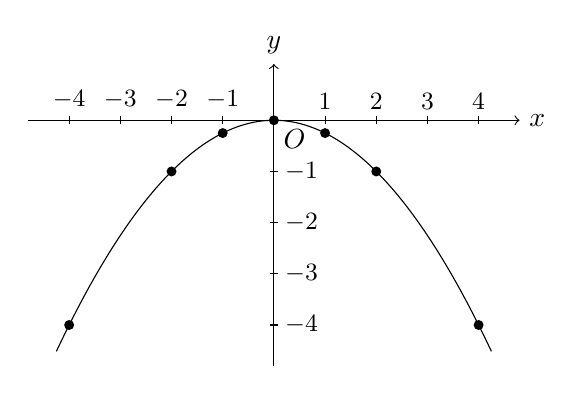
\begin{tikzpicture}[x=0.65cm,y=0.65cm]
        \draw[->] (-4.8,0) -- (4.8,0) node[right] {$x$};
        \draw[->] (0,-4.8) -- (0,1.1) node[above] {$y$};
        \foreach \x in {-4,-3,-2,-1,1,2,3,4}
            \draw (\x,0.08)--(\x,-0.08) node[above=2pt] {\small $\x$};
        \foreach \y in {-4,-3,-2,-1}
            \draw (0.08,\y)--(-0.08,\y) node[right=2pt] {\small $\y$};
        \draw[domain=-4.25:4.25,samples=81,smooth,variable=\x]
            plot ({\x},{-0.25*(\x)^2});
        \foreach \x/\y in {-4/-4,-2/-1,-1/-0.25,0/0,1/-0.25,2/-1,4/-4}
            \fill (\x,\y) circle[radius=1.8pt];
        \node[below right] at (0,0) {$O$};
    \end{tikzpicture}

    \textit{Hình 6.2}
    \end{center}

    \textbf{Nhận biết tính đối xứng của đồ thị hàm số $y=ax^2$ ($a\ne0$)}

    \textbf{HĐ4.} Xét đồ thị của hàm số $y=2x^2$ đã vẽ ở HĐ3 (H.6.3).
    \begin{enumerate}[label=\alph*)]
        \item Đồ thị nằm phía trên hay phía dưới trục hoành? Điểm nào là điểm thấp nhất của đồ thị?
        \item So sánh hoành độ và tung độ của các cặp điểm thuộc đồ thị: $A(1;2)$ và $A'(-1;2)$; $B(2;8)$ và $B'(-2;8)$. Từ đó hãy nhận xét mối liên hệ về vị trí giữa các cặp điểm nêu trên.
        \item Tìm điểm $C$ có hoành độ $x=\dfrac{1}{2}$ thuộc đồ thị. Xác định tọa độ của điểm $C'$ đối xứng với điểm $C$ qua trục tung $Oy$ và cho biết điểm $C'$ có thuộc đồ thị đã cho hay không.
    \end{enumerate}

    \begin{center}
    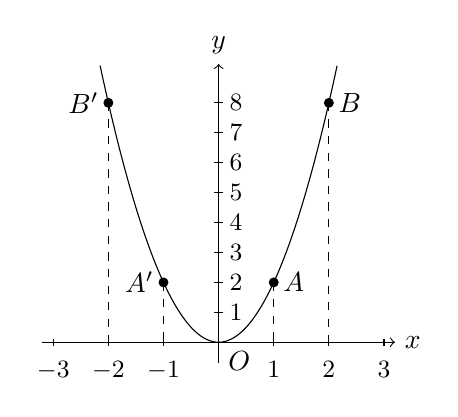
\begin{tikzpicture}[x=0.7cm,y=0.38cm]
        \draw[->] (-3.2,0) -- (3.2,0) node[right] {$x$};
        \draw[->] (0,-0.7) -- (0,9.3) node[above] {$y$};
        \foreach \x in {-3,-2,-1,1,2,3}
            \draw (\x,0.12)--(\x,-0.12) node[below=2pt] {\small $\x$};
        \foreach \y in {1,2,3,4,5,6,7,8}
            \draw (0.08,\y)--(-0.08,\y) node[right=2pt] {\small $\y$};
        \draw[domain=-2.15:2.15,samples=81,smooth,variable=\x]
            plot ({\x},{2*(\x)^2});
        \coordinate (Ap) at (-1,2);
        \coordinate (A) at (1,2);
        \coordinate (Bp) at (-2,8);
        \coordinate (B) at (2,8);
        \draw[dashed] (Ap)--(-1,0) (A)--(1,0) (Bp)--(-2,0) (B)--(2,0);
        \fill (Ap) circle[radius=1.8pt] node[left] {$A'$};
        \fill (A) circle[radius=1.8pt] node[right] {$A$};
        \fill (Bp) circle[radius=1.8pt] node[left] {$B'$};
        \fill (B) circle[radius=1.8pt] node[right] {$B$};
        \node[below right] at (0,0) {$O$};
    \end{tikzpicture}

    \textit{Hình 6.3}
    \end{center}

    \begin{keyconcept}
        Đồ thị của hàm số $y=ax^2$ ($a\ne0$) là một đường cong, gọi là \textbf{đường parabol}, có các tính chất sau:
        \begin{itemize}
            \item Có đỉnh là gốc tọa độ $O$;
            \item Có trục đối xứng là $Oy$;
            \item Nằm phía trên trục hoành nếu $a>0$ và nằm phía dưới trục hoành nếu $a<0$.
        \end{itemize}
    \end{keyconcept}

    Hai điểm $(x;y)$ và $(-x;y)$ đối xứng nhau qua trục tung $Oy$.

    \begin{center}
    \begin{tikzpicture}[x=0.75cm,y=0.75cm]
        \begin{scope}[xshift=-2.4cm]
            \draw[->] (-2.2,0)--(2.2,0) node[right] {$x$};
            \draw[->] (0,-0.5)--(0,3.0) node[above] {$y$};
            \draw[domain=-1.8:1.8,samples=61,smooth,variable=\x]
                plot ({\x},{0.8*(\x)^2});
            \node[below left] at (0,0) {$O$};
            \node[above left] at (-1.6,2.2) {$a>0$};
        \end{scope}
        \begin{scope}[xshift=2.4cm]
            \draw[->] (-2.2,0)--(2.2,0) node[right] {$x$};
            \draw[->] (0,-3.0)--(0,0.8) node[above] {$y$};
            \draw[domain=-1.8:1.8,samples=61,smooth,variable=\x]
                plot ({\x},{-0.8*(\x)^2});
            \node[above right] at (0,0) {$O$};
            \node[above left] at (-1.6,0.45) {$a<0$};
        \end{scope}
    \end{tikzpicture}

    \textit{Hình 6.4. Đồ thị của hàm số $y=ax^2$ ($a\ne0$)}
    \end{center}

    \textbf{Ví dụ 3.}
    \begin{enumerate}[label=\alph*)]
        \item Vẽ đồ thị của hàm số $y=-2x^2$.
        \item Tìm tọa độ các điểm thuộc đồ thị có tung độ bằng $-\dfrac{1}{2}$ và nhận xét về tính đối xứng giữa các điểm đó.
    \end{enumerate}

    \textbf{Giải}

    a) Lập bảng một số giá trị tương ứng giữa $x$ và $y$:

    \begin{center}
    \begin{tblr}{
        colspec={Q[c] *{5}{Q[c]}},
        rows={0.9cm}
    }
        $x$ & $-2$ & $-1$ & $0$ & $1$ & $2$ \\
        $y=-2x^2$ & $-8$ & $-2$ & $0$ & $-2$ & $-8$ \\
    \end{tblr}
    \end{center}

    Biểu diễn các điểm $(-2;-8)$, $(-1;-2)$, $(0;0)$, $(1;-2)$ và $(2;-8)$ trên mặt phẳng tọa độ $Oxy$ và nối chúng lại ta được đồ thị của hàm số $y=-2x^2$ như Hình 6.5.

    \begin{center}
    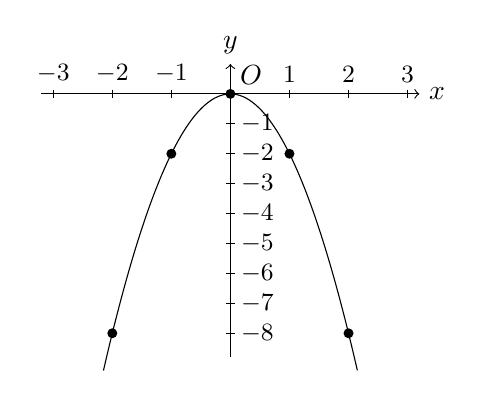
\begin{tikzpicture}[x=0.75cm,y=0.38cm]
        \draw[->] (-3.2,0)--(3.2,0) node[right] {$x$};
        \draw[->] (0,-8.8)--(0,1.0) node[above] {$y$};
        \foreach \x in {-3,-2,-1,1,2,3}
            \draw (\x,0.14)--(\x,-0.14) node[above=2pt] {\small $\x$};
        \foreach \y in {-8,-7,-6,-5,-4,-3,-2,-1}
            \draw (0.08,\y)--(-0.08,\y) node[right=2pt] {\small $\y$};
        \draw[domain=-2.15:2.15,samples=81,smooth,variable=\x]
            plot ({\x},{-2*(\x)^2});
        \foreach \x/\y in {-2/-8,-1/-2,0/0,1/-2,2/-8}
            \fill (\x,\y) circle[radius=1.8pt];
        \node[above right] at (0,0) {$O$};
    \end{tikzpicture}

    \textit{Hình 6.5}
    \end{center}

    b) Ta có: $y=-\dfrac{1}{2}$ nên $-2x^2=-\dfrac{1}{2}$, hay $x^2=\dfrac{1}{4}$. Suy ra $x=\dfrac{1}{2}$ hoặc $x=-\dfrac{1}{2}$.

    Vậy có hai điểm cần tìm là $\left(\dfrac{1}{2};-\dfrac{1}{2}\right)$ và $\left(-\dfrac{1}{2};-\dfrac{1}{2}\right)$. Hai điểm này đối xứng với nhau qua trục tung $Oy$.

    \textbf{Nhận xét.}
    \begin{itemize}
        \item Khi vẽ đồ thị hàm số $y=ax^2$ ($a\ne0$), ta cần xác định tối thiểu $5$ điểm thuộc đồ thị là gốc tọa độ $O$ và hai cặp điểm đối xứng với nhau qua trục tung $Oy$.
        \item Do đồ thị của hàm số $y=ax^2$ ($a\ne0$) nhận trục tung $Oy$ là trục đối xứng nên ta có thể lập bảng giá trị của hàm số này với những giá trị $x$ không âm và vẽ phần đồ thị tương ứng ở bên phải trục tung, sau đó lấy đối xứng phần đồ thị đã vẽ qua trục tung ta sẽ được đồ thị của hàm số đã cho.
    \end{itemize}

    \textbf{Luyện tập 2.} Vẽ đồ thị của hàm số $y=\dfrac{1}{2}x^2$. Tìm các điểm thuộc đồ thị có tung độ bằng $2$ và nhận xét về tính đối xứng giữa các điểm đó.

    \answerline
    \answerline
    \answerline

    \textbf{Vận dụng 2.} Giải quyết bài toán ở \textit{tình huống mở đầu}.

    \answerline
    \answerline
\end{lesson}

\begin{exercises}
    \subsection{Bài tập}

    \begin{questions}[series=SGK]
        \item Cho hàm số $y=0{,}25x^2$. Hoàn thành bảng giá trị sau vào vở:

        \begin{center}
        \begin{tblr}{
            colspec={Q[c] *{7}{Q[c]}},
            rows={0.9cm}
        }
            $x$ & $-3$ & $-2$ & $-1$ & $0$ & $1$ & $2$ & $3$ \\
            $y$ & & & & & & & \\
        \end{tblr}
        \end{center}

        \item Cho hình lăng trụ đứng có đáy là hình vuông cạnh $a$ (cm) và chiều cao $10$ cm.
        \begin{questions}
            \item Viết công thức tính thể tích $V$ của hình lăng trụ theo $a$ và tính giá trị của $V$ khi $a=2$ cm.
            \item Nếu độ dài cạnh đáy tăng lên hai lần thì thể tích của hình lăng trụ thay đổi thế nào?
        \end{questions}
        \answerline
        \answerline

        \item Diện tích toàn phần $S$ (cm$^2$) của một hình lập phương, tức là tổng diện tích xung quanh và diện tích của hai mặt đáy là một hàm số của độ dài cạnh $a$ (cm).
        \begin{questions}
            \item Viết công thức của hàm số này.
            \item Sử dụng công thức nhận được ở câu a để tính độ dài cạnh của một hình lập phương có diện tích toàn phần là $54$ cm$^2$.
        \end{questions}
        \answerline
        \answerline

        \item Vẽ đồ thị của các hàm số sau:
        \begin{questions}
            \item $y=3x^2$;
            \item $y=-\dfrac{1}{3}x^2$.
        \end{questions}
        \answerline
        \answerline
        \answerline

        \item Biết rằng đường cong trong Hình 6.6 là một parabol $y=ax^2$.
        \begin{questions}
            \item Tìm hệ số $a$.
            \item Tìm tung độ của điểm thuộc parabol có hoành độ $x=-2$.
            \item Tìm các điểm thuộc parabol có tung độ $y=8$.
        \end{questions}

        \begin{center}
        \begin{tikzpicture}[x=0.7cm,y=0.5cm]
            \draw[step=1,base100] (-4.5,-0.4) grid (4.6,8.8);
            \draw[->] (-4.8,0)--(4.9,0) node[right] {$x$};
            \draw[->] (0,-0.6)--(0,9.0) node[above] {$y$};
            \foreach \x in {-4,-3,-2,-1,1,2,3,4}
                \draw (\x,0.1)--(\x,-0.1) node[below=2pt] {\small $\x$};
            \foreach \y in {1,2,3,4,5,6,7,8}
                \draw (0.08,\y)--(-0.08,\y) node[left=2pt] {\small $\y$};
            \draw[domain=-4.2:4.2,samples=81,smooth,variable=\x]
                plot ({\x},{0.5*(\x)^2});
            \foreach \x/\y in {-2/2,-1/0.5,1/0.5,2/2}
                \fill (\x,\y) circle[radius=1.8pt];
            \node[below right] at (0,0) {$O$};
            \node[right] at (1,0.5) {$0{,}5$};
        \end{tikzpicture}

        \textit{Hình 6.6}
        \end{center}

        \answerline
        \answerline

        \item Trong Hình 6.7 có hai đường cong là đồ thị của hai hàm số $y=-3x^2$ và $y=x^2$. Hãy cho biết đường nào là đồ thị của hàm số $y=-3x^2$.

        \begin{center}
        \begin{tikzpicture}[x=0.75cm,y=0.75cm]
            \draw[->] (-3.5,0)--(3.5,0) node[right] {$x$};
            \draw[->] (0,-3.5)--(0,4.8) node[above] {$y$};
            \foreach \x in {-3,-2,-1,1,2,3}
                \draw (\x,0.08)--(\x,-0.08) node[below=2pt] {\small $\x$};
            \foreach \y in {-3,-2,-1,1,2,3,4}
                \draw (0.08,\y)--(-0.08,\y) node[left=2pt] {\small $\y$};
            \draw[domain=-2.15:2.15,samples=81,smooth,variable=\x]
                plot ({\x},{(\x)^2});
            \draw[domain=-1.15:1.15,samples=81,smooth,variable=\x]
                plot ({\x},{-3*(\x)^2});
            \node[below left] at (0,0) {$O$};
        \end{tikzpicture}

        \textit{Hình 6.7}
        \end{center}

        \answerline

        \item Một cổng vòm được thiết kế dạng parabol $y=ax^2$ như Hình 6.8. Biết chiều rộng của chân cổng là $AB=6$ m và chiều cao của cổng là $OI=4{,}5$ m.

        \begin{center}
        \begin{tikzpicture}[x=0.85cm,y=0.85cm]
            \coordinate (O) at (0,0);
            \coordinate (I) at (0,-4.5);
            \coordinate (A) at (-3,-4.5);
            \coordinate (B) at (3,-4.5);
            \coordinate (H) at (2,-4.5);
            \coordinate (K) at (2,-2);
            \draw[->] (-4.2,0)--(4.8,0) node[right] {$x$};
            \draw[->] (0,-5.0)--(0,1.0) node[above] {$y$};
            \draw[domain=-3.2:3.2,samples=81,smooth,variable=\x]
                plot ({\x},{-0.5*(\x)^2});
            \draw[dashed] (A)--(3,-4.5) (A)--(-3,0) (B)--(3,0) (H)--(K);
            \foreach \x in {-4,-3,-2,-1,1,2,3,4}
                \draw (\x,0.08)--(\x,-0.08) node[above=2pt] {\small $\x$};
            \foreach \y in {-4,-3,-2,-1}
                \draw (0.08,\y)--(-0.08,\y) node[left=2pt] {\small $\y$};
            \fill (O) circle[radius=1.8pt] node[above right] {$O$};
            \fill (A) circle[radius=1.8pt] node[below] {$A$};
            \fill (B) circle[radius=1.8pt] node[below] {$B$};
            \fill (I) circle[radius=1.8pt] node[below] {$I$};
            \fill (H) circle[radius=1.8pt] node[below] {$H$};
            \fill (K) circle[radius=1.8pt] node[right] {$K$};
            \node[right] at (3.55,-4.5) {\textit{Mặt đất}};
            \draw[<->] (3.75,0)--(3.75,-4.5) node[midway,right] {$4{,}5$ m};
            \draw[<->] (0,-4.9)--(2,-4.9) node[midway,below] {$2$ m};
            \node[right] at (2.05,-3.2) {$x$};
        \end{tikzpicture}

        \textit{Hình 6.8}
        \end{center}

        \begin{questions}
            \item Tìm hệ số $a$ dựa vào các dữ kiện trên. Từ đó, tính độ dài đoạn $HK$ biết $H$ cách điểm chính giữa cổng $I$ là $2$ m.
            \item Để vận chuyển hàng qua cổng, người ta dự định sử dụng một xe tải có chiều rộng $2$ m, chiều cao $3$ m. Hỏi xe tải này có thể đi qua được cổng vòm đó hay không?
        \end{questions}
        \answerline
        \answerline
        \answerline
    \end{questions}
\end{exercises}

\begin{practice}
    \subsection{Luyện tập}

    \begin{questions}[series=SBT]
        \item Thể tích $V$ của hình lăng trụ đứng tứ giác có đáy là hình vuông và chiều cao $5$ cm là một hàm số của độ dài cạnh đáy $a$ (cm).
        \begin{questions}
            \item Viết công thức của hàm số này và tính độ dài cạnh đáy của hình lăng trụ nếu biết thể tích bằng $180$ cm$^3$.
            \item Nếu độ dài cạnh $a$ của hình vuông đáy tăng lên hai lần thì thể tích $V$ của khối lăng trụ thay đổi như thế nào?
        \end{questions}
        \answerline
        \answerline

        \item Cầu treo Sunshine Skyway bắc qua Vịnh Tampa ở bang Florida (Mỹ), được hỗ trợ bởi $21$ dây cáp làm bằng thép, mỗi dây có đường kính $9$ inch. Khối lượng mà mỗi dây cáp có thể chịu được là $w=8d^2$ (tấn), trong đó $d$ là đường kính của dây cáp (tính bằng inch) (Theo \textit{Algebra 2, NXB McGraw-Hill, 2018}).
        \begin{questions}
            \item Tính khối lượng tối đa mà cây cầu treo có thể chịu đựng được.
            \item Nếu muốn cây cầu treo có thể chịu được khối lượng là $15\,162$ tấn thì đường kính của dây cáp phải là bao nhiêu?
        \end{questions}
        \answerline
        \answerline

        \item Lực $F$ của gió khi thổi vuông góc vào cánh buồm tỉ lệ thuận với bình phương tốc độ $v$ của gió, tức là $F=av^2$ ($a$ là hằng số). Biết rằng khi tốc độ gió bằng $2$ m/s thì lực tác động lên cánh buồm của một chiếc thuyền bằng $120$ N.
        \begin{questions}
            \item Tính hằng số $a$.
            \item Hỏi khi tốc độ gió $v=15$ m/s thì lực thổi $F$ của gió bằng bao nhiêu?
            \item Biết rằng cánh buồm chỉ có thể chịu được một áp lực tối đa là $12\,000$ N, hỏi chiếc thuyền có thể đi được trong gió bão với tốc độ gió $90$ km/h không?
        \end{questions}
        \answerline
        \answerline
        \answerline

        \item Xác định hệ số $a$ của hàm số $y=ax^2$ ($a\ne0$), biết đồ thị của hàm số đi qua điểm:
        \begin{questions}
            \item $A\left(-\dfrac{1}{2};-\dfrac{3}{2}\right)$;
            \item $B\left(\dfrac{1}{2};\dfrac{\sqrt{3}}{4}\right)$.
        \end{questions}
        \answerline
        \answerline

        \item Trong hình bên có đồ thị của ba hàm số $y=-2x^2$, $y=x^2$, $y=2x^2$.
        \begin{questions}
            \item Cho biết đường nào là đồ thị của hàm số $y=-2x^2$.
            \item Trong hai đường còn lại, với mỗi $x$ hãy so sánh hai giá trị tương ứng của $y$ để phân biệt đồ thị hai hàm số $y=x^2$ và $y=2x^2$.
        \end{questions}

        \begin{center}
        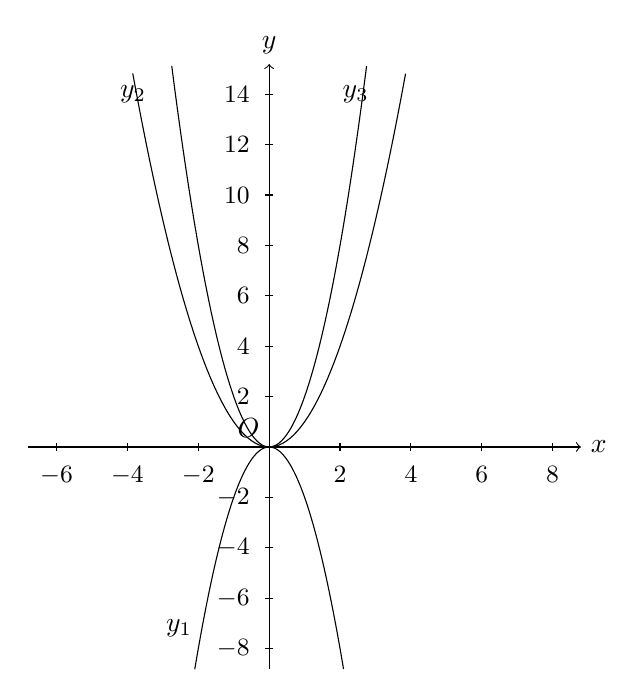
\begin{tikzpicture}[x=0.45cm,y=0.32cm]
            \draw[->] (-6.8,0)--(8.8,0) node[right] {$x$};
            \draw[->] (0,-8.8)--(0,15.2) node[above] {$y$};
            \foreach \x in {-6,-4,-2,2,4,6,8}
                \draw (\x,0.15)--(\x,-0.15) node[below=2pt] {\small $\x$};
            \foreach \y in {-8,-6,-4,-2,2,4,6,8,10,12,14}
                \draw (0.12,\y)--(-0.12,\y) node[left=2pt] {\small $\y$};
            \draw[domain=-2.75:2.75,samples=81,smooth,variable=\x]
                plot ({\x},{2*(\x)^2});
            \draw[domain=-3.85:3.85,samples=81,smooth,variable=\x]
                plot ({\x},{(\x)^2});
            \draw[domain=-2.1:2.1,samples=81,smooth,variable=\x]
                plot ({\x},{-2*(\x)^2});
            \node[left] at (-1.9,-7.2) {$y_1$};
            \node[left] at (-3.2,14.0) {$y_2$};
            \node[right] at (1.8,14.0) {$y_3$};
            \node[above left] at (0,0) {$O$};
        \end{tikzpicture}
        \end{center}

        \answerline
        \answerline

        \item Trên cùng một mặt phẳng tọa độ $Oxy$, vẽ parabol $(P):y=-x^2$ và đường thẳng $(d):y=x-2$. Dùng đồ thị xác định tọa độ các giao điểm của hai đường này.
        \answerline
        \answerline
        \answerline

        \item Vẽ đồ thị của hai hàm số sau trên cùng một mặt phẳng tọa độ:
        \[
            y=0{,}75x^2;\qquad y=-0{,}75x^2.
        \]
        Có nhận xét gì về vị trí của hai đồ thị này so với trục hoành $Ox$?
        \answerline
        \answerline
        \answerline

        \item Cho hàm số $y=f(x)=ax^2$ ($a\ne0$).
        \begin{questions}
            \item Chứng tỏ rằng nếu $(x_0;y_0)$ là một điểm thuộc đồ thị hàm số thì điểm $(-x_0;y_0)$ cũng nằm trên đồ thị hàm số đó.
            \item Chứng minh rằng $f(-x)=f(x)$ với mọi $x$ thuộc $\mathbb{R}$.
        \end{questions}
        \answerline
        \answerline
        \answerline
    \end{questions}
\end{practice}
